\documentclass{article}

\usepackage{defines}

\usepackage{tikz}
\usetikzlibrary{tikzmark, calc}

\begin{document}

\tickettitle{3}{Конечные и бесконечные множества. Счётные множества, их свойства.}

\define{конечного множества}

Непустое множество $M$ называется конечным, если:
\begin{align*}
	\exists n\in\N:\exists f:M\leftrightarrow\setdef{x\in\N}{x\leq n}
\end{align*}

$\setdef{x\in\N}{x\leq n}$ --- отрезок натурального ряда.

$\eset$ --- конечное множество.

Если множество не конечно, то оно бесконечно.

$\N$ --- простейшее бесконечное множество.

\define{счётного множества}

Множество $X$ счётно, если $\exists f:X\leftrightarrow \N$. Иначе $X$ несчётно.

Примеры счётных множеств: $\N, \mathbb{Q}$

\sectitle{Свойства счётных множеств}

\theorem

$A$ --- счётно $\Rarr$ $B \subset A$ --- конечно или счётно.

\proof
\begin{align*}
	 & A=\setdef{a_i}{i\in\N} \Rarr B=\{a_{n_i}\} \land (n_{i+1}>n_i)                 \\
	 & \exists \text{наибольшее }n_i\Rarr B \text{ --- конечно, иначе --- счётно}\qed
\end{align*}

\theorem

Объединение $\forall$ конечного или счётного числа счётных множеств --- счётное множество

\proof
\begin{align*}
	 & A_1: a_{11}\tikzmark{a11},\;\;a_{12}\tikzmark{a12},\;\;a_{13}\tikzmark{a13},\;\;... \\[1.2ex]
	 & A_2: a_{21}\tikzmark{a21},\;\;a_{22}\tikzmark{a22},\;\;...                          \\[1.2ex]
	 & A_3: a_{31}\tikzmark{a31},\;\;...                                                   \\
	 & ...
	\begin{tikzpicture}[remember picture, overlay]
		\draw [-latex] ($(pic cs:a11)+(0,0.3em)$) -- ($(pic cs:a12)+(-1.5em,0.3em)$);
		\draw [-latex] ($(pic cs:a12)+(-1.5em,0.1em)$) -- ($(pic cs:a21)+(-0.7em,0.5em)$);
		\draw [-latex] ($(pic cs:a21)+(-1em,-0.1em)$) -- ($(pic cs:a31)+(-1em,0.6em)$);
		\draw [-latex] ($(pic cs:a31)+(-0.7em,0.5em)$) -- ($(pic cs:a22)+(-1.5em,0.1em)$);
		\draw [-latex] ($(pic cs:a22)+(-0.7em,0.5em)$) -- ($(pic cs:a13)+(-1.5em,0.1em)$);
		\draw [-latex] ($(pic cs:a13)+(0,0.3em)$) -- ($(pic cs:a13)+(1em,0.3em)$);
	\end{tikzpicture}
\end{align*}

Нумеруя $\bigcup_i A_i$ по диагонали мы получаем $f:\bigcup_i A_i\leftrightarrow\N\qed$

\pagebreak

\theorem

$\forall$ бесконечное множество $M$ содержит счётное подмножество.

\proof
\begin{align*}
	\sqsupset a_1                 & \in M                                           \\
	\exists a_2                   & \in M:a_2\neq a_1                               \\
	(\forall n\in\N)\;\exists a_n & \in M: a_n \neq a_i\;\forall i=\overline{1,n-1} \\
	A:=\setdef{a_i}{i\in\N}       & \subset M\qed                                   \\
\end{align*}

\end{document}
